
\documentclass{standalone}
\usepackage[svgnames]{xcolor}
\usepackage{pgfplots}
\pgfplotsset{compat=newest}
\usepackage[sfdefault]{FiraSans}
\usepackage{FiraMono}
\renewcommand*\familydefault{\sfdefault}
\begin{document}
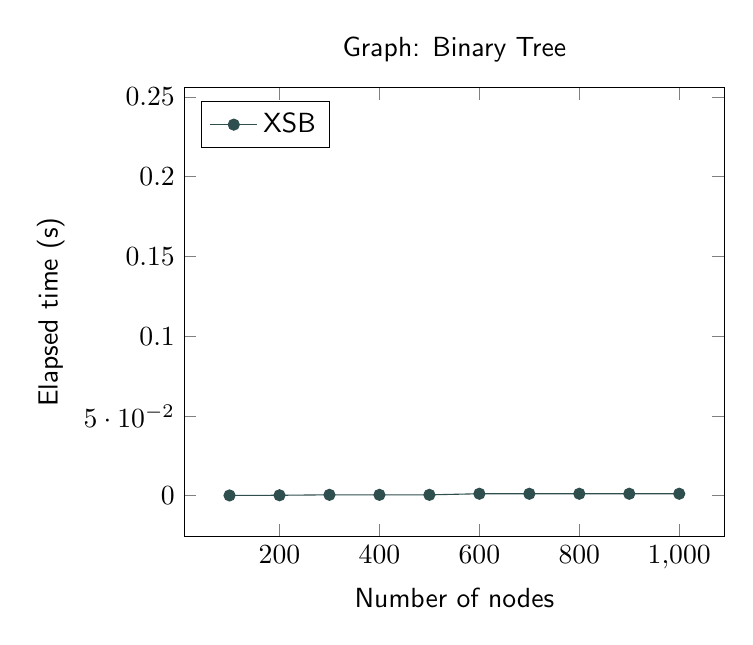
\begin{tikzpicture}
    \begin{axis}[
        title={Graph: Binary Tree},
        xlabel={Number of nodes},
        ylabel={Elapsed time (s)},
        legend pos={north west},
        ymax=0.2557331163901836
    ]
    \addplot+[DarkSlateGray, mark options={color=DarkSlateGray}] coordinates {(100,7.920265197753909e-05) (200,0.0001856327056884766) (300,0.0004714012145996092) (400,0.000461244583129883) (500,0.00045647621154785154) (600,0.001146221160888674) (700,0.001135015487670896) (800,0.0011425495147705078) (900,0.001141452789306642) (1000,0.00114603042602539)};
\addlegendentry{XSB}

    \end{axis}
\end{tikzpicture}
\end{document}
